\subsection{Оптические вычислители}\label{sec:OpticalCalcs}
Один из методов решения проблем описанных в \ref{sec:ANN} - это делегирование отдельных задач отдельным вычислительным единицам. Как правило, подобные вычислительные единицы направлены на решение более узкого спектра задач. Это позволяет эффективно изменить их архитектуру и способ работы с памятью. Ярким примером такого решения является графический процессор (ГП). Его основная задача - это параллельная обработка большого массива данных. На рисунке \ref{ris:PerfomanceGPUCPU} подразумевается максимальная скорость вычислений, поэтому его можно использовать для сравнения производительности процессоров и графических процессоров в параллельных задачах. Видно, что разрыв производительности составляет от 2 до 8 раз, в зависимости от конкретной линейки процессоров.
\par
Последнее время набирает популярность использование оптических устройств для ускорения или увеличение эффективности исполнения задач. Такие вычислители являются аналоговыми, чаще всего, выполняют очень узкий спектр задач на скорости ограниченной лишь электронными частями схемы \cite{solli2015analog}, могут предоставлять высокий параллелизм за счёт ортогональности излучения с различными длинами волн \cite{mcmahon2023physics}, а также, могут обеспечить низкое энергопотребление \cite{wu2022analog}. Существуют множество исследований и оптических схем, выполняющих особые задачи.





\paragraph{Оптические корреляторы}
Оптический коррелятор - это оптическое устройство  производящая свёртку изображения с ядром. Существуют два основных метода оптической свёртки $4f$ схема - VLC (Vander Lugt Correlator) коррелятор \cite{lugt1964signal}, изображённый на рисунке \ref{ris:VLC} из \cite{goncharov2019features}, и JTC (Joint Trnsform Correlator) коррелятор \cite{weaver1966technique}, изображённый на рисунке \ref{ris:VLC} из \cite{alfalou2009optical}.
\begin{figure}[h]
	\centering{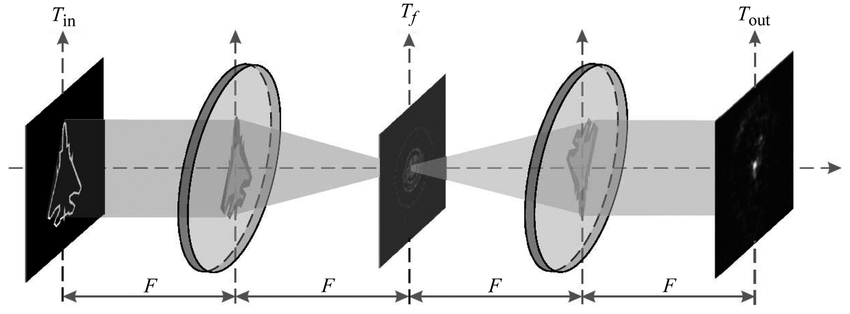
\includegraphics[width=0.8\linewidth]{figures/VLC.png}}
	\caption{Оптическая схема VLC коррелятора.}
	\label{ris:VLC}
\end{figure}
\begin{figure}[h]
	\centering{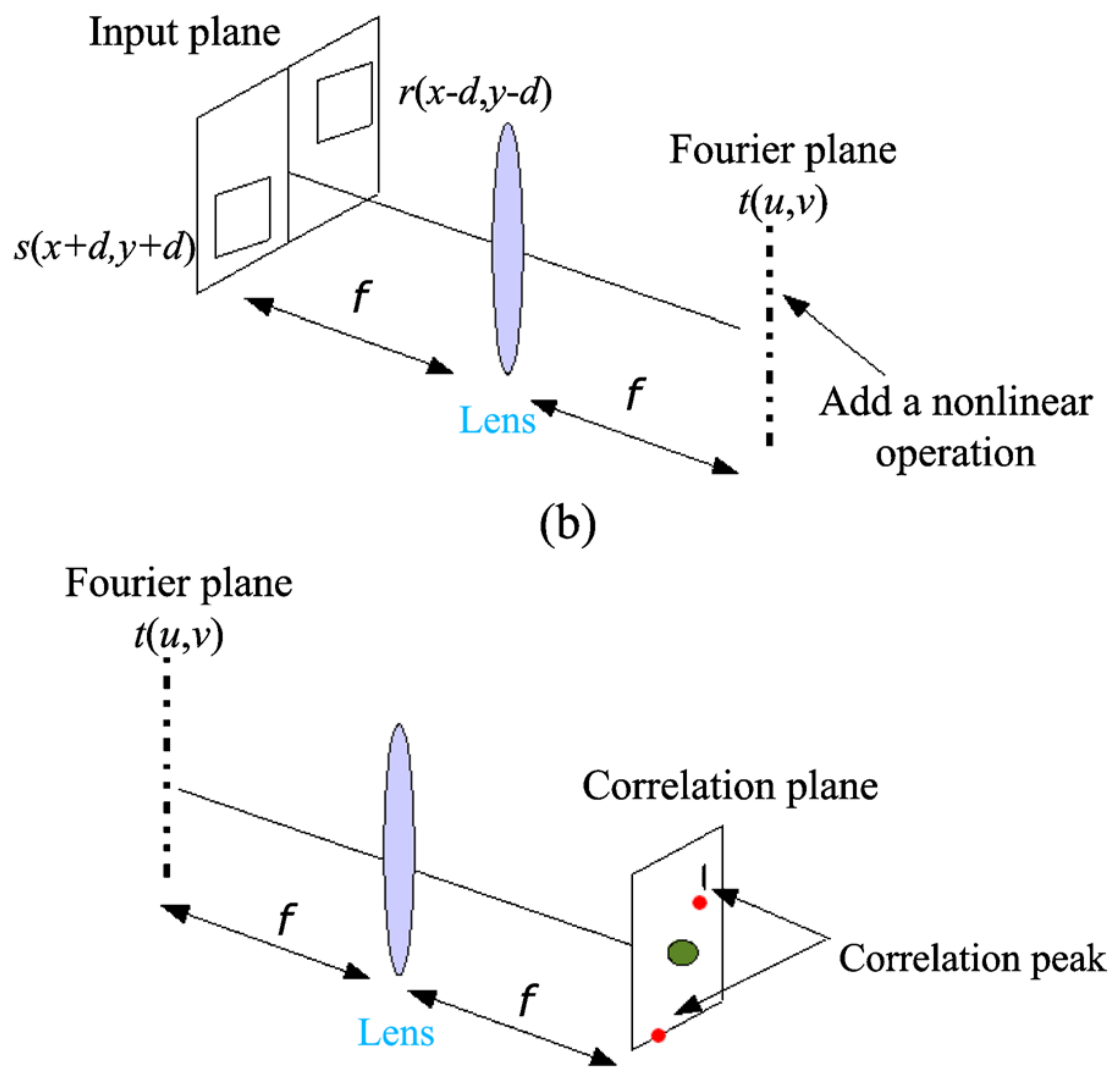
\includegraphics[width=0.65\linewidth]{figures/JTC.png}}
	\caption{Оптическая схема JTC коррелятора.}
	\label{ris:JTC}
\end{figure}
Принцип работы VLC коррелятора основан на теореме о свёртке, которая гласит, что свёртка двух функций - это обратное Фурье преобразование произведения их Фурье образов. В этой схеме, первая линза создаёт Фурье образ \cite{goodman2005introduction} на некотором модуляторе, на нём изображение умножается на Фурье образ ядра, а потом, вторая линза делает ещё одно преобразование Фурье, что эквивалентно, отражению вдоль каждой оси обратному Фурье преобразованию.
Принцип работы JTC коррелятора основан на том, что нелинейная функция от Фурье образа совмещённого изображения содержит член, пропорциональный произведению этих Фурье образов. Математические выражения доказывающие это приведены в последовательности уравнений \ref{eq:JTC}.
\begin{equation}\label{eq:JTC}
	\tiny{\begin{matrix}
		\left|\mathcal{F}\left(f(x,y) + g(x-b,y)\right)\right|^2 
		=
		\left|\mathcal{F}\left(f(x,y)\right) + \mathcal{F}\left(g(x,y)\right)e^{-ik_xb}\right|^2
		=
		\\
		\left|\mathcal{F}\left(f(x,y)\right)\right|^2
		+
		\left|\mathcal{F}\left(g(x,y)\right)\right|^2
		+
		\mathcal{F}\left(f(x,y)\right)\mathcal{F}\left(g(x,y)\right)^*e^{+ik_xb}
		+
		\mathcal{F}\left(f(x,y)\right)^*\mathcal{F}\left(g(x,y)\right)e^{-ik_xb}
		\\
		\text{Учтём}
		\\
		\mathcal{F}^{-1}\left(
			\left|\mathcal{F}\left(f(x,y)\right)\right|^2
		\right)
		=
		\mathcal{F}^{-1}\left(
			\mathcal{F}\left(f(x,y)\right)\mathcal{F}\left(f^*(x,y)\right)
		\right)
		=
		f(x,y) \bullet f^*(x,y)
		\\
		\mathcal{F}^{-1}\left(
			\mathcal{F}\left(f(x,y)\right)\mathcal{F}\left(g(x,y)\right)^*e^{+ik_xb}
		\right)
		=
		(f(x,y) \bullet g^*(x,y))(x+b,y)
		\\
		\text{Итоговое выражение}
		\\
		\left(f(x,y) \bullet f^*(x,y) + g(x,y) \bullet g^*(x,y)\right)
		+ (f(x,y) \bullet g^*(x,y))(x+b,y) + (f^*(x,y) \bullet g(x,y))(x-b,y)
	\end{matrix}}
\end{equation}





\paragraph{Оптическое сжатие информации}
Статья \cite{alfalou2009optical} содержит обзор множества методов сжатия информации с помощью оптики. В основном, все методы основаны на свёртки изображений с теми фильтрами, т.е. разложение изображения по некоторому набору функций. Эта  концепция важна, например, если мы хотим сжимать фотографии из некоторого набора, в котором изображены объекты с похожими признаками, то можно найти такой набор функций, который содержит меньше мод чем система, по которой можно однозначно восстановить любое изображение, но при эти функции такие, что изображения из набора восстанавливаются однозначно.

\FloatBarrier\par
В статье \cite{alkholidi2008real} обсуждается замена операции свёртки с вейвлетами в преобразовании JPEG2000 \cite{lawson2002image}, на оптическую реализацию. В качестве вейвлетов использовались вейвлеты Хаара, вид которых представлен в уравнении \ref{eq:HaarVevlet}.
\begin{equation}\label{eq:HaarVevlet}
	\begin{matrix}
		\varphi_{LL} = 
			\left(\begin{matrix} 
				+\frac{1}{2} && +\frac{1}{2} \\ +\frac{1}{2} && +\frac{1}{2} 
			\end{matrix}\right)
		&&
		\varphi_{HL} = 
		\left(\begin{matrix} 
			+\frac{1}{2} && +\frac{1}{2} \\ -\frac{1}{2} && -\frac{1}{2} 
		\end{matrix}\right)
		\\
		\varphi_{LH} = 
		\left(\begin{matrix} 
			+\frac{1}{2} && -\frac{1}{2} \\ +\frac{1}{2} && -\frac{1}{2} 
		\end{matrix}\right)
		&&
		\varphi_{HH} = 
		\left(\begin{matrix} 
			+\frac{1}{2} && -\frac{1}{2} \\ -\frac{1}{2} && +\frac{1}{2} 
		\end{matrix}\right)
	\end{matrix}
\end{equation}
Свёртка изображения с $\varphi_{HH}$ выделяет низкие частоты, с $\varphi_{HL}$ - высокие частоты по горизонтали и низкие по вертикале, с $\varphi_{LH}$ - высокие по вертикале и низкие по горизонтали, с $\varphi_{LL}$ - высокие частоты. Оптически свёртка с каждым ядром производилось по отдельности путём перемножения Фурье образа изображения с Фурье образом ядра в $4f$. Дублирование изображение на четыре копии производится с помощью периодической голограммы. После свёртки с вейвлетами Хаара, результаты фокусируются на матрице камеры. Дальнейшие шаги сжатия заключаются в уменьшении количество уровней дискретизации интенсивности сигналов пикселей матрицы и изменении кодировки для уменьшения количества информации. Схема этой оптической схемы изображена на графике \ref{ris:JPEG2000}. Результаты численных расчётов работы такой схемы изображены на рисунке \ref{ris:VLCERMSSNR}.
\begin{figure}[h]
	\centering{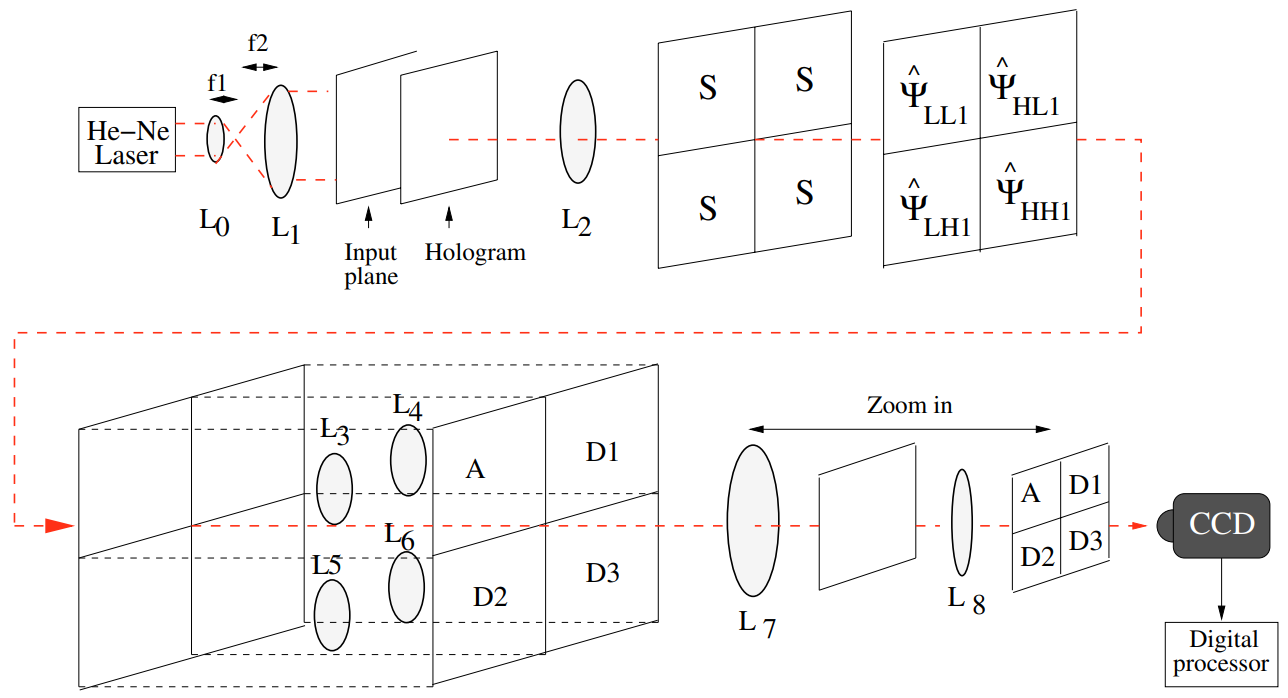
\includegraphics[width=0.8\linewidth]{figures/JPEG2000.png}}
	\caption{Оптическая схема реализации свёртки вейвлетами Хаара.}
	\label{ris:JPEG2000}
\end{figure}
\begin{figure}[h]
	\centering
		\begin{minipage}{.40\textwidth}
			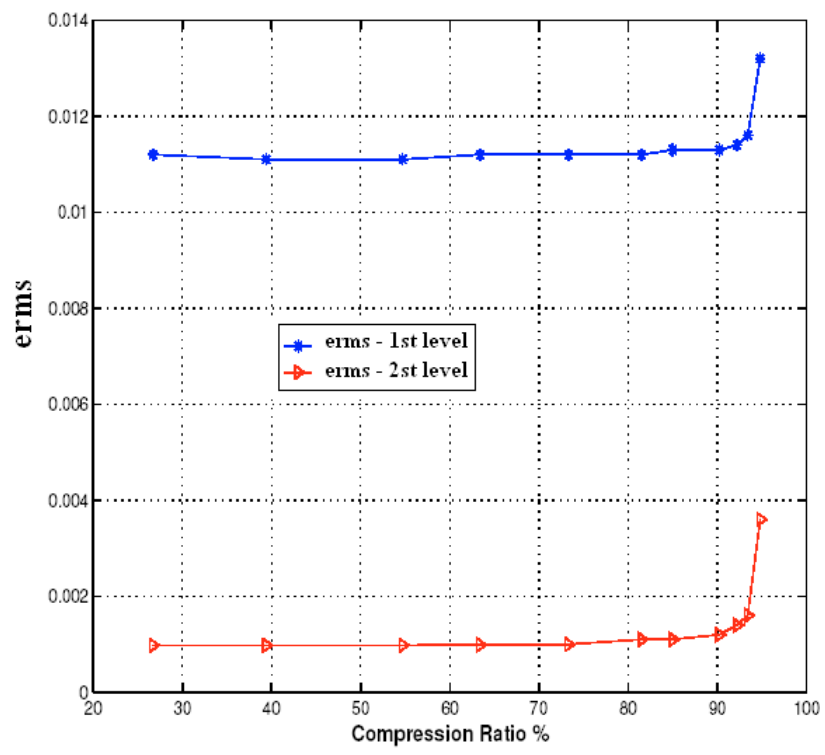
\includegraphics[width=\linewidth]{figures/VLCERMS.png}
			\label{ris:VLCERMS}
		\end{minipage}
		\hfill
		\begin{minipage}{.40\textwidth}
			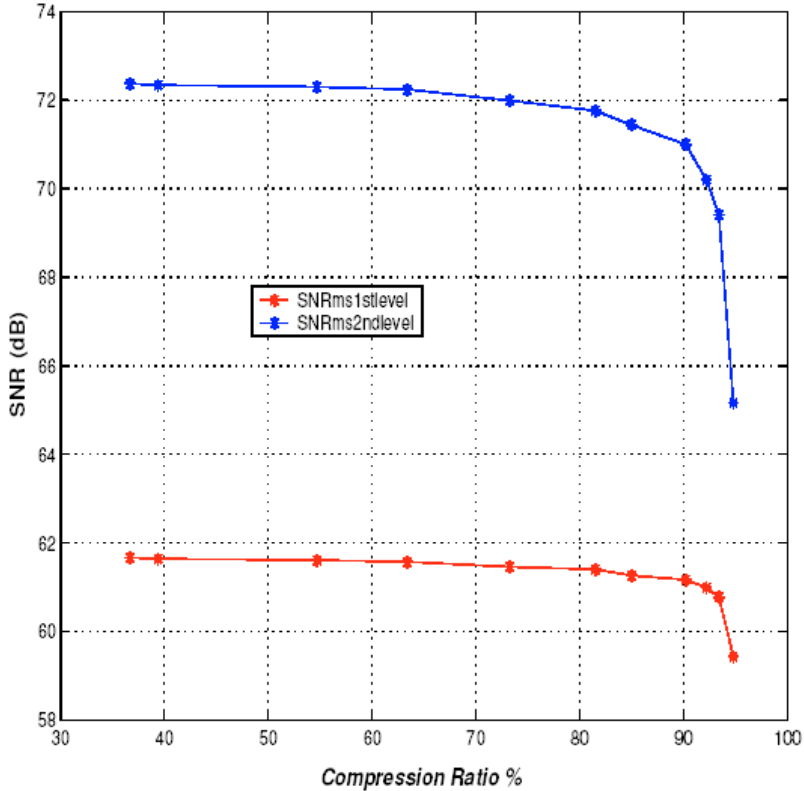
\includegraphics[width=0.95\linewidth]{figures/VLCSNR.png}
			\label{ris:VLCSNR}
		\end{minipage}
		\caption{Средне квадратичное отклонение значений пикселей и соотношения сигнал-шум в зависимости от степени сжатия метода с оптической свёрткой с вейвлетами Хаара \cite{alkholidi2008real}. Красная и синяя линии соответствую первому и второму уровню отношению размера ядра к размеру изображения.}
		\label{ris:VLCERMSSNR}
\end{figure}

\FloatBarrier\par
В статье \cite{alkholidi2007new} представлен оптический метод сжатия изображений, основанный на замене косинусного преобразованием в алгоритме JPEG оптической частью. Основная идея заключается в отражении изображения по двум осям, приводя его к чётному виду и последующему получению Фурье образа с помощью линзы \cite{goodman2005introduction}, и последующего обрезания определённых частот. Схема этого метода изображена на рисунке \ref{ris:JPEG}. Результаты численных расчётов представлены в таблице \ref{ris:JPEGres}. Результаты эксперимента для степени сжатия на рисунке \ref{ris:JPEGres2}.
\begin{figure}[h]
	\centering{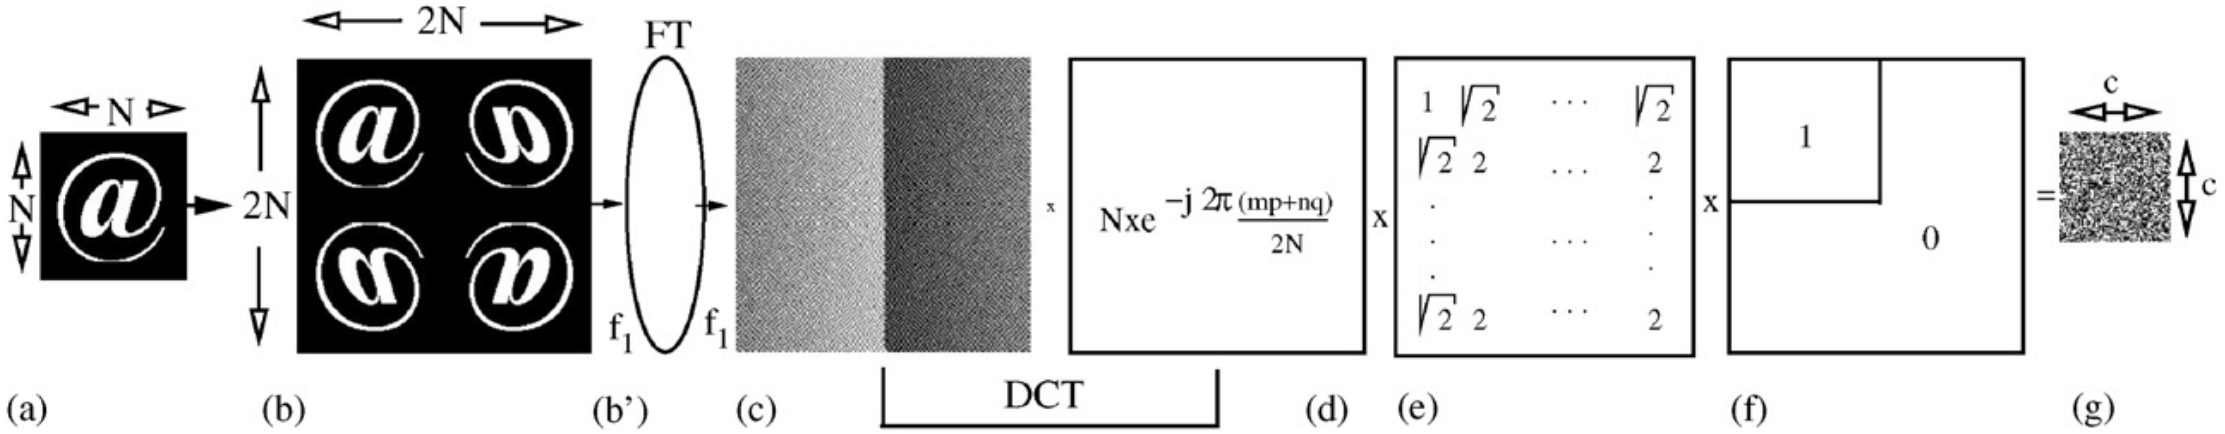
\includegraphics[width=0.8\linewidth]{figures/JPEG.png}}
	\caption{Принципиальная схема оптического косинусного преобразования и последующего обрезания частот.}
	\label{ris:JPEG}
\end{figure}
\begin{figure}[h]
	\centering{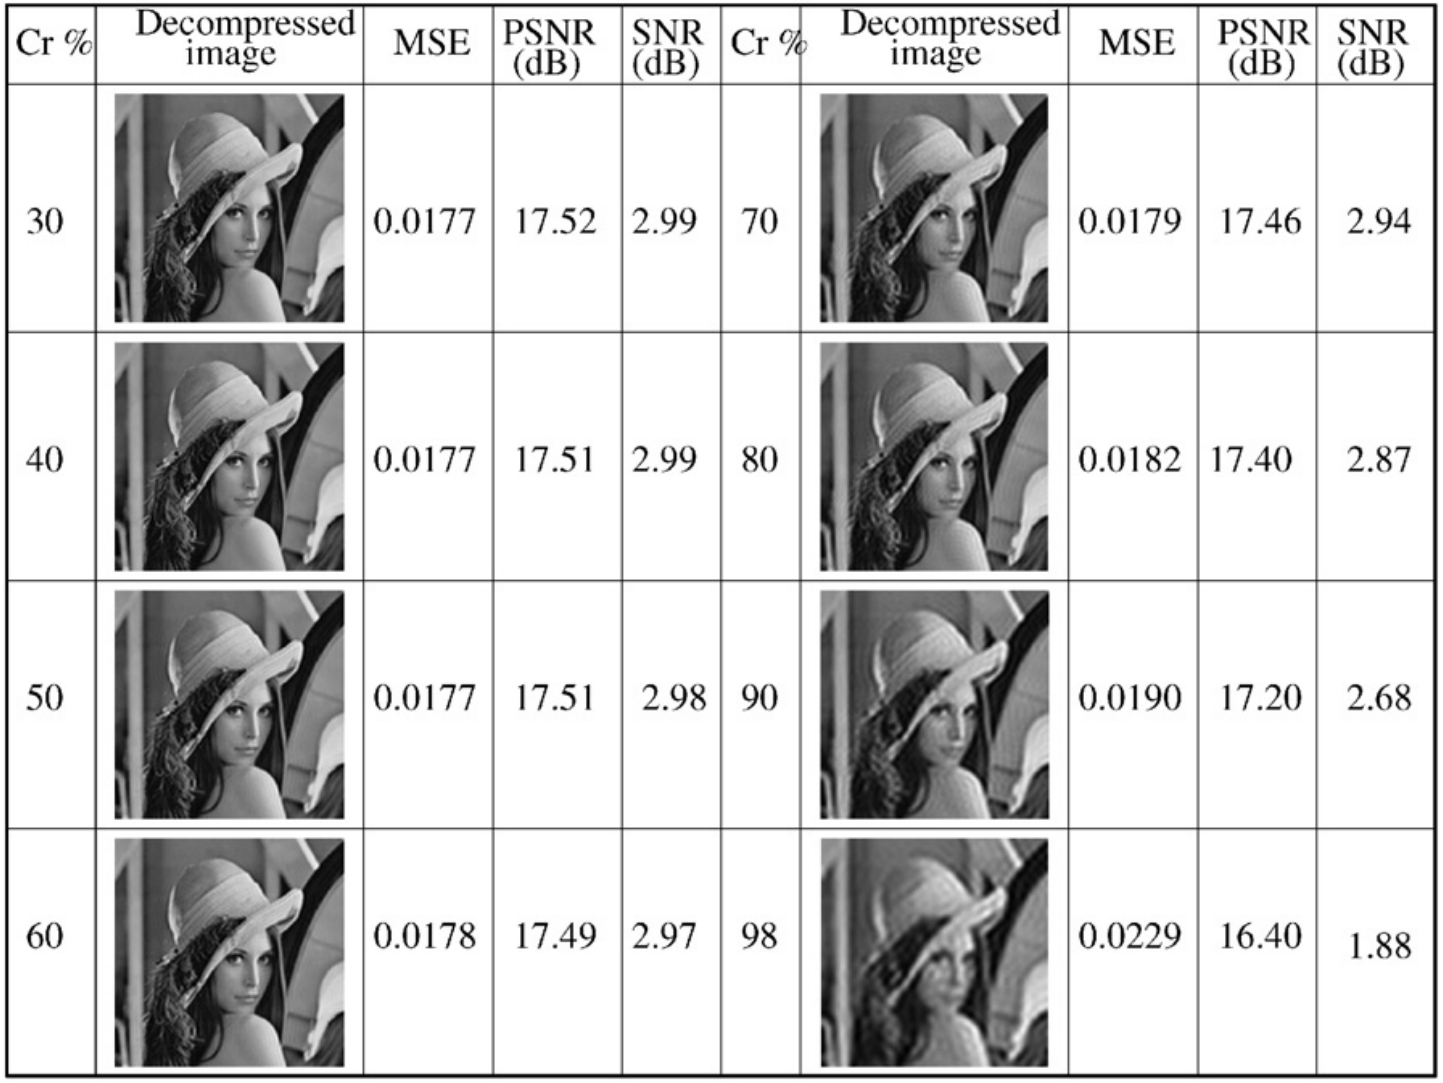
\includegraphics[width=0.7\linewidth]{figures/JPEGres.png}}
	\caption{Результаты симуляции сжатия изображения при помощи оптического косинусного преобразования и последующего восстановления.}
	\label{ris:JPEGres}
\end{figure}
\begin{figure}[h]
	\centering{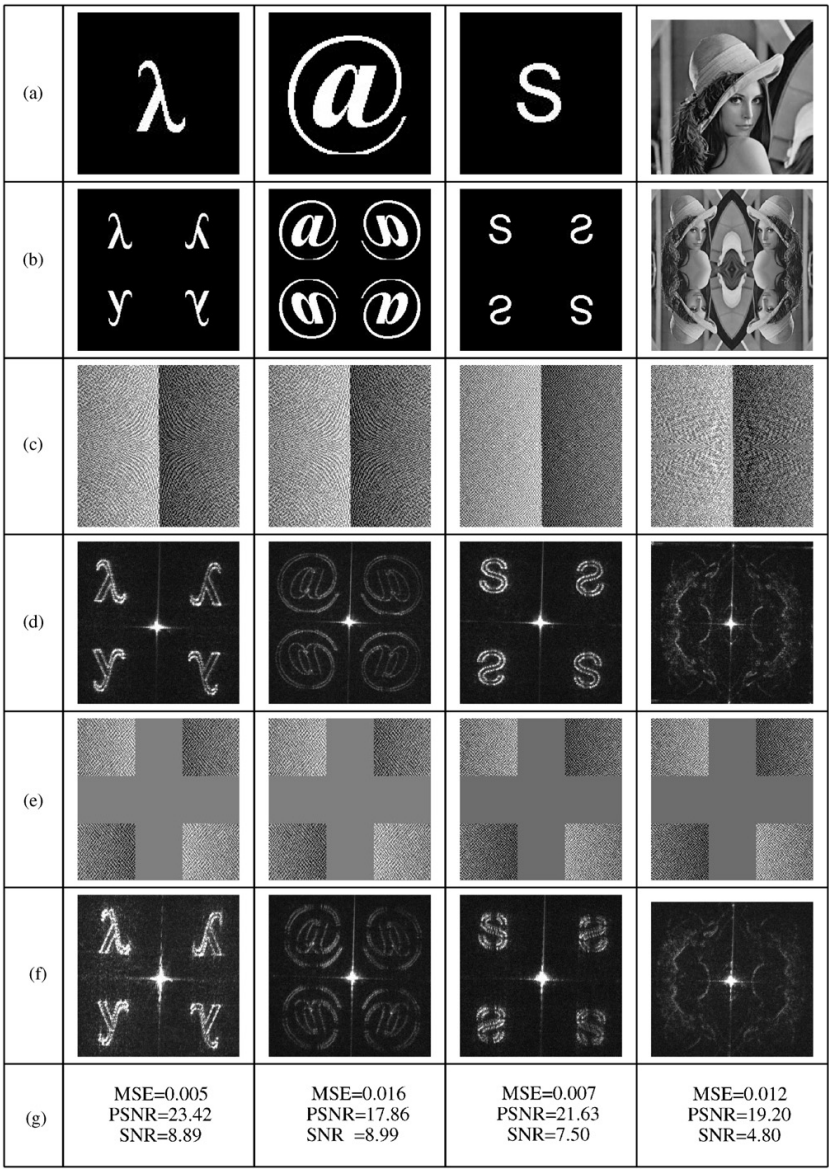
\includegraphics[angle=90,width=0.9\linewidth]{figures/JPEGres2.png}}
	\caption{Результаты оптической реализации сжатия и декомпрессии JPEG (Степень сжатия $50\%$): (a) исходное изображение; (b) реплицированное изображение; (c) реплицированный спектр изображения; (d) оптическая плоскость вывода; (e) сжатый спектр; (f) декомпрессированное изображение; (g) оценка между (b) и (f).}
	\label{ris:JPEGres2}
\end{figure}
Сравнивая численные расчёты (рисунок \ref{ris:JPEGres}) и эксперимент (рисунок \ref{ris:JPEGres2}) становится понятно, что данный оптический метод сжатия очень плохо работает с не разреженными изображениями. Также, можно заметить, что не всякая мера сравнения изображений соотносится с наблюдаемой реальностью. Среднеквадратичная ошибка для картинки в 4-ом столбце в эксперименте меньше чем в симуляции для соответствующей степени сжатия $50\%$, но очевидно, что в эксперименте картинка восстановилась намного хуже.

\FloatBarrier\par
В статье \cite{velez2016optical} использовался JTC коррелятор для свёртки изображения со случайной матрицей и последующее оптическое масштабирование этой свёртки, описанное в \cite{trejos2016optical}. Основа этого метода лежит в методике сжатия разреженных данных с помощью случайных проекций \cite{amador2007random}. Суть заключается в разложение изображения по случайным, заранее заданным, функциям. Результат численных расчётов работы этой схемы изображён на рисунке \ref{ris:RandomProjRes}.
\begin{figure}[h]
	\centering{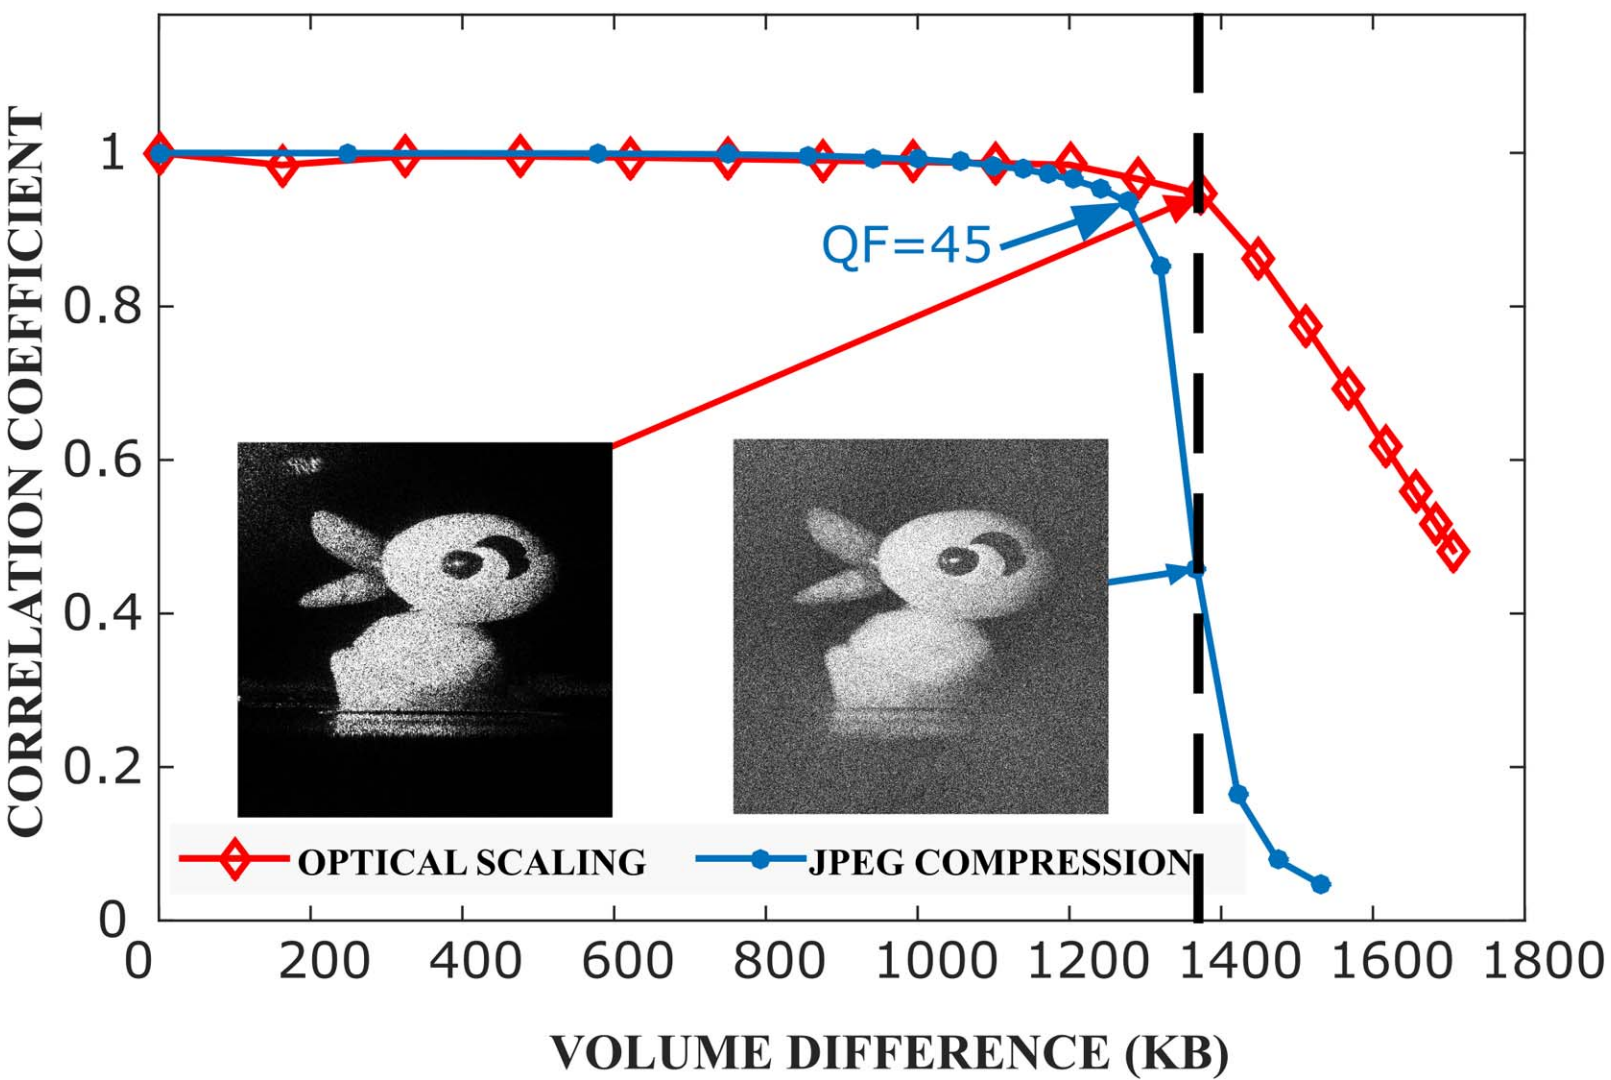
\includegraphics[width=0.8\linewidth]{figures/RandomProjRes.png}}
	\caption{Коэффициент корреляции между объектом, восстановленным из несжатых и сжатых данных поля для оптического масштабирования и сжатия JPEG, с точки зрения разницы в объеме.}
	\label{ris:RandomProjRes}
\end{figure}





\paragraph{Дифракционные нейронные сети}
Дифракционная нейронная сеть представляет массив оптически неоднородных тонких масок. На каждой такой маске по точечно модулируется фаза и(или) амплитуда поля. Такую систему ассоциируют с нейронной сетью типа перцептрон потому, что поле в каждой точке плоскости линейно связано с полями точек в предыдущей плоскости. Важным отличием является тот факт, что количество весов перехода между слоями намного меньше. Это связано с тем фактом, что поле в какой-то точке, вычисляется как интеграл поля в предыдущей плоскости, перемноженного на фиксированное ядро, и последующее умножения этого числа на управляемый коэффициент (формула \ref{eq:FieldProp}).
\begin{equation}\label{eq:FieldProp}
	u_i(x,y) = w_i(x,y)\int\limits_{-\infty}^{+\infty}\int\limits_{-\infty}^{+\infty}u_{i-1}(\xi,\eta)\frac{e^{ik\sqrt{L^2+(x-\xi)^2+(y-\eta)^2}}}{\sqrt{L^2+(x-\xi)^2+(y-\eta)^2}} d\xi d\eta
\end{equation}
В этом уравнение $u_i,u_{i-1}$ поле в текущем и предыдущем слое соответственно, $L$ - расстояние между слоями, $w_i(x,y)$ - вес нейрона в точке $x,y$, а количество нейронов и дискретизация этого уравнения определяется степенью точности с которой можно создавать оптические неоднородности.
Таким образом, на один переход между слоями размером $N$ нейронов, перцептрон имеет $N^2$ весов, а дифракционная нейронная сеть - $N$.

\FloatBarrier\par
Классическая реализация дифракционной нейронной сети представлена в статье \cite{qian2020performing}. На рисунке \ref{ris:ClassicD2NN} изображена оптическая схема эксперимента. В этой работе использовалось излучение с длинной волны $17.6$мм. Оптическая нейронная сеть выполняла логические операции (НЕ, И, ИЛИ). Выбор операции и двух входных сигналов производился за счёт первой плоскости, далее шли два скрытых слоя, состоящих из параллелепипедов различной высоты, на каждом из которых излучение получало различные добавки к фазе. На выходной плоскости значениям $0$ и $1$ соответствовали две разные области фокусировки. Высота каждого параллелепипеда оптимизировалась с помощью методов машинного обучения. 
\begin{figure}[h]
	\centering{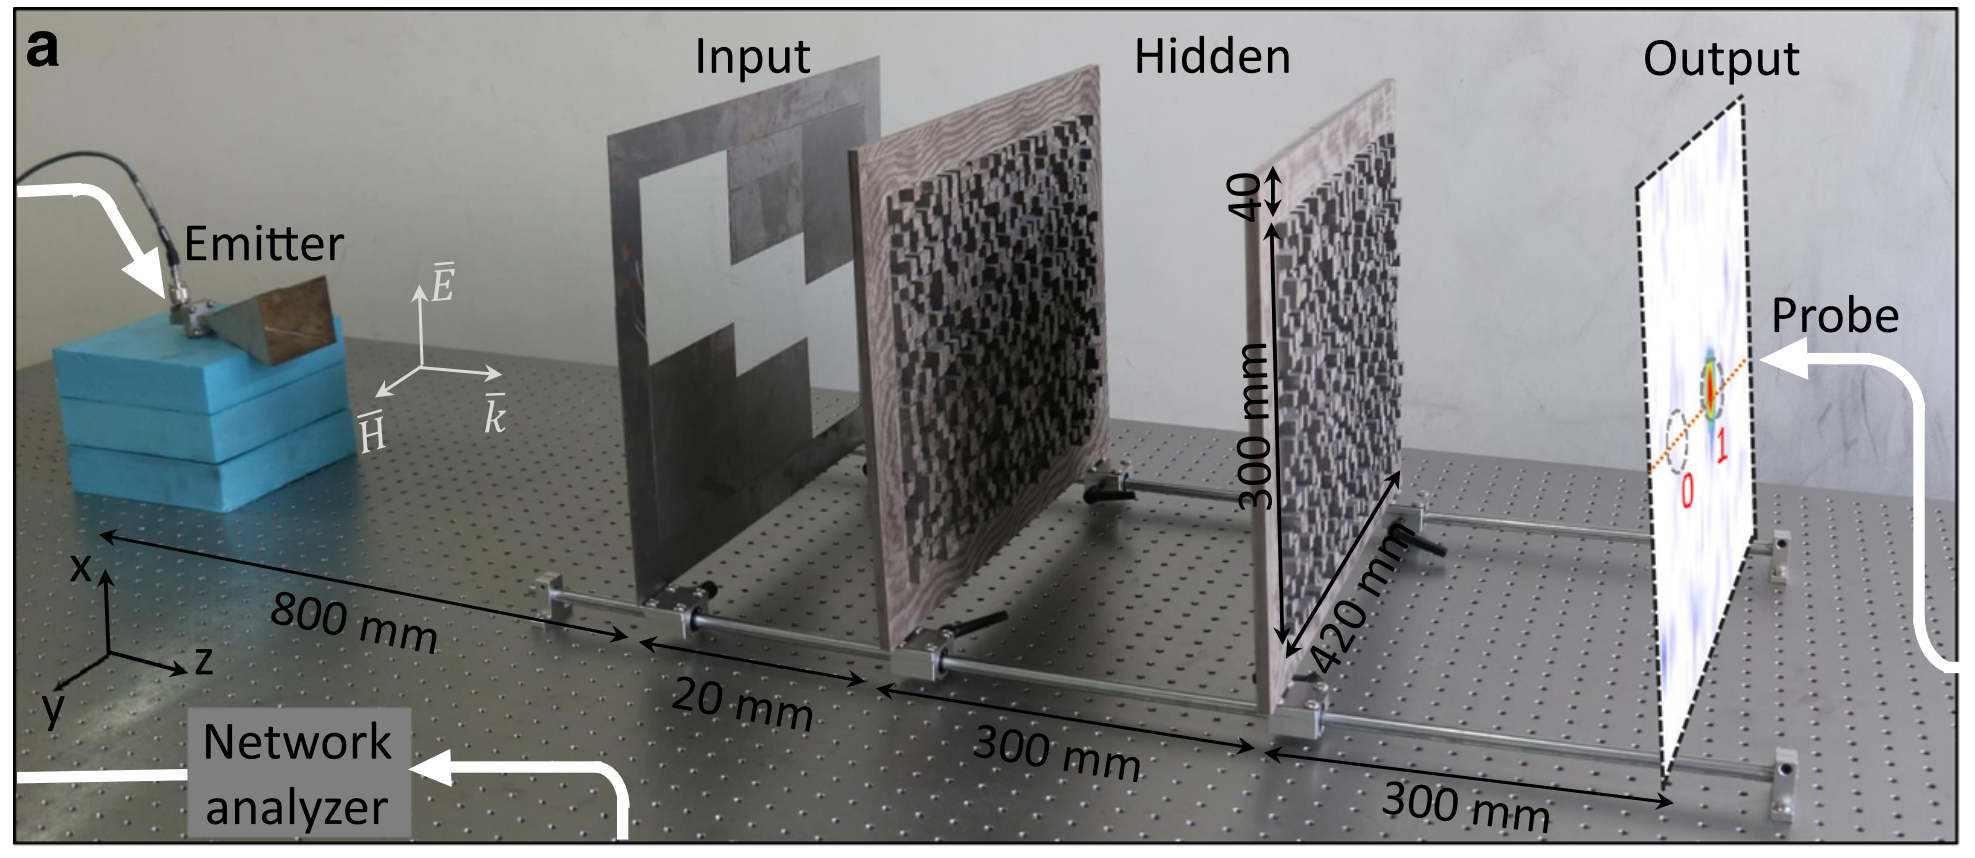
\includegraphics[width=0.8\linewidth]{figures/ClassicD2NN.png}}
	\caption{Экспериментальная реализация дифракционной нейронной сети из статьи \cite{qian2020performing}.}
	\label{ris:ClassicD2NN}
\end{figure}
Исследователи смогли обучить подобную нейронную сеть так, что она выполняла указанные выше операции без ошибок.

\FloatBarrier\par
Сравнение других, более сложных, реализаций представлено в статье \cite{yan2019fourier}. В этой схемы, протестированные в этой работе, представлены на графике \ref{ris:FD2NN} в схематическом виде. Сеть обучалась на классификацию рукописных цифр и должна была направить результирующие поле в один из десяти детекторов, соответствующих цифрам $0$-$9$. Внизу находятся графики результатов их обучения.
\begin{figure}[h]
	\centering{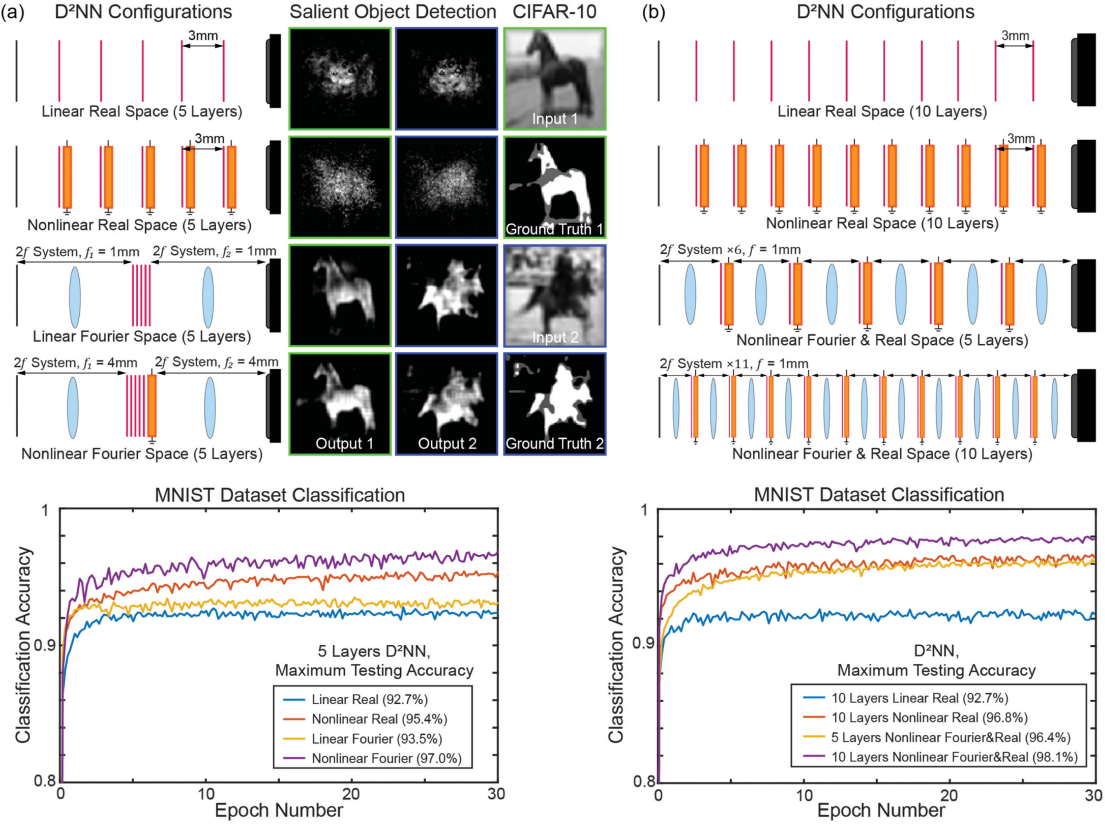
\includegraphics[width=0.8\linewidth]{figures/FD2NN.png}}
	\caption{Схемы дифракционных нейронных сетей (сверху) и результаты их обучения (снизу) \cite{yan2019fourier}.}
	\label{ris:FD2NN}
\end{figure}





% \paragraph{Гибридные оптоэлектронные сети}

